\section{Experimental overview of Bottomonia results at RHIC and LHC}

%\subsubsection{Proton-proton collisions as a reference for R$_{AA}$ at the LHC}


\subsection{$\Upsilon$(nS) R$_{AA}$}

\paragraph{Measurement by CMS, ATLAS and ALICE}

The bottomonia states ($\Upsilon$(nS)) are measured at the LHC with very good statistical
precision~\cite{Chatrchyan:2012lxa,Abelev:2014nua,Chatrchyan:2011pe,Khachatryan:2016xxp}.
The CMS measurements at $\sNN =$2.76 TeV~\cite{Chatrchyan:2012lxa,Chatrchyan:2011pe} reveal
a clear proof of sequential suppression :  $\Upsilon$(2S) and $\Upsilon$(3S) are 
more suppressed relative to the ground state $\Upsilon$(1S).   The individual $\Upsilon$ states are also found to be suppressed in
the PbPb collisions relative to the production in the pp collisions. The $\Upsilon$ nuclear
modification factor, $R_{AA}$, shows a strong dependence on collision centrality but has
weak dependence on $\Upsilon$ meson $\pT$ and rapidity~\cite{Khachatryan:2016xxp}.
The forward rapidity ($2.5 \leq y^{\Upsilon} \leq 4.0$) measurement of the $\Upsilon$ suppression at 
ALICE~\cite{Abelev:2014nua} is found to be consistent with the midrapidity ($|y^{\Upsilon}|\,\leq 2.4$)
measurement of the $\Upsilon$ suppression at the CMS. 
The CMS and ALICE collaborations have carried out the $R_{AA}$ measurement of $\Upsilon$
at $\sNN =$ 5.02 TeV with the Run II LHC PbPb
collisions~\cite{Sirunyan:2018nsz,Sirunyan:2017lzi,ALICE:2018wzm}.
The CMS experiment measured slightly more amount of $\Upsilon$ suppression at
$\sNN =$ 5.02 TeV~\cite{Sirunyan:2018nsz,Sirunyan:2017lzi} than the suppression at
$\sNN =$ 2.76 TeV~\cite{Khachatryan:2016xxp} while the ALICE experiment observed less
suppression at $\sNN =$ 5.02 TeV than that at $\sNN =$ 2.76 TeV 
in the most central PbPb collisions~\cite{Abelev:2014nua,ALICE:2018wzm}. 


\begin{figure}
  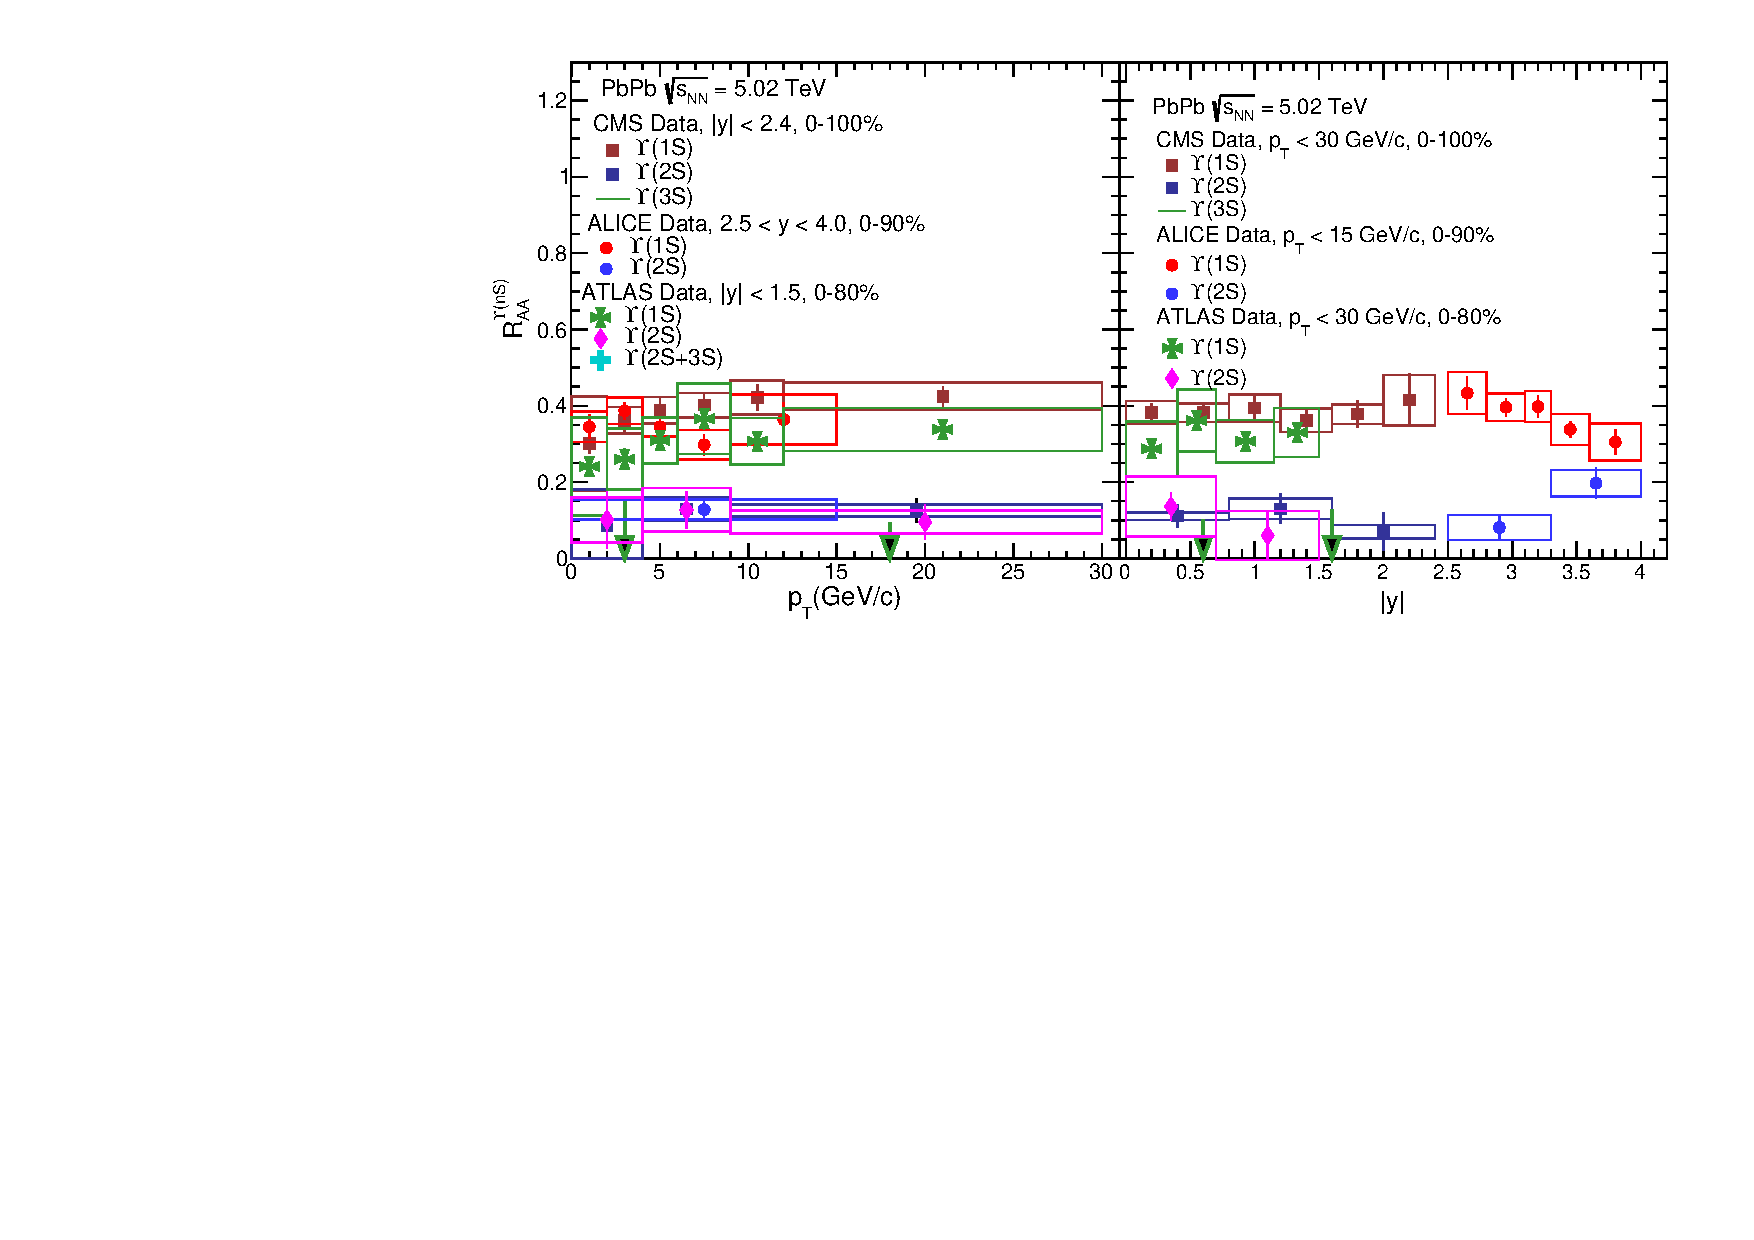
\includegraphics[width=0.99\textwidth]{Figures/ExpOverview/Fig_LHC_YnSRAAPtRap.pdf}
  \caption{(Color online) The $\Upsilon$(nS) nuclear modification factor, $R_{AA}$, (a) as a function of transverse momentum $p_{T}$
    and (b) as a function of rapidity measured by CMS~\cite{CMS:2018zza} and ALICE experiments~\cite{ALICE:2020wwx}. The vertical bars denote statistical uncertainties, and the rectangular boxes show the total systematic uncertainties.
  }
  \label{fig:LHCYnSRAAPtRap}
\end{figure}


\begin{figure}
  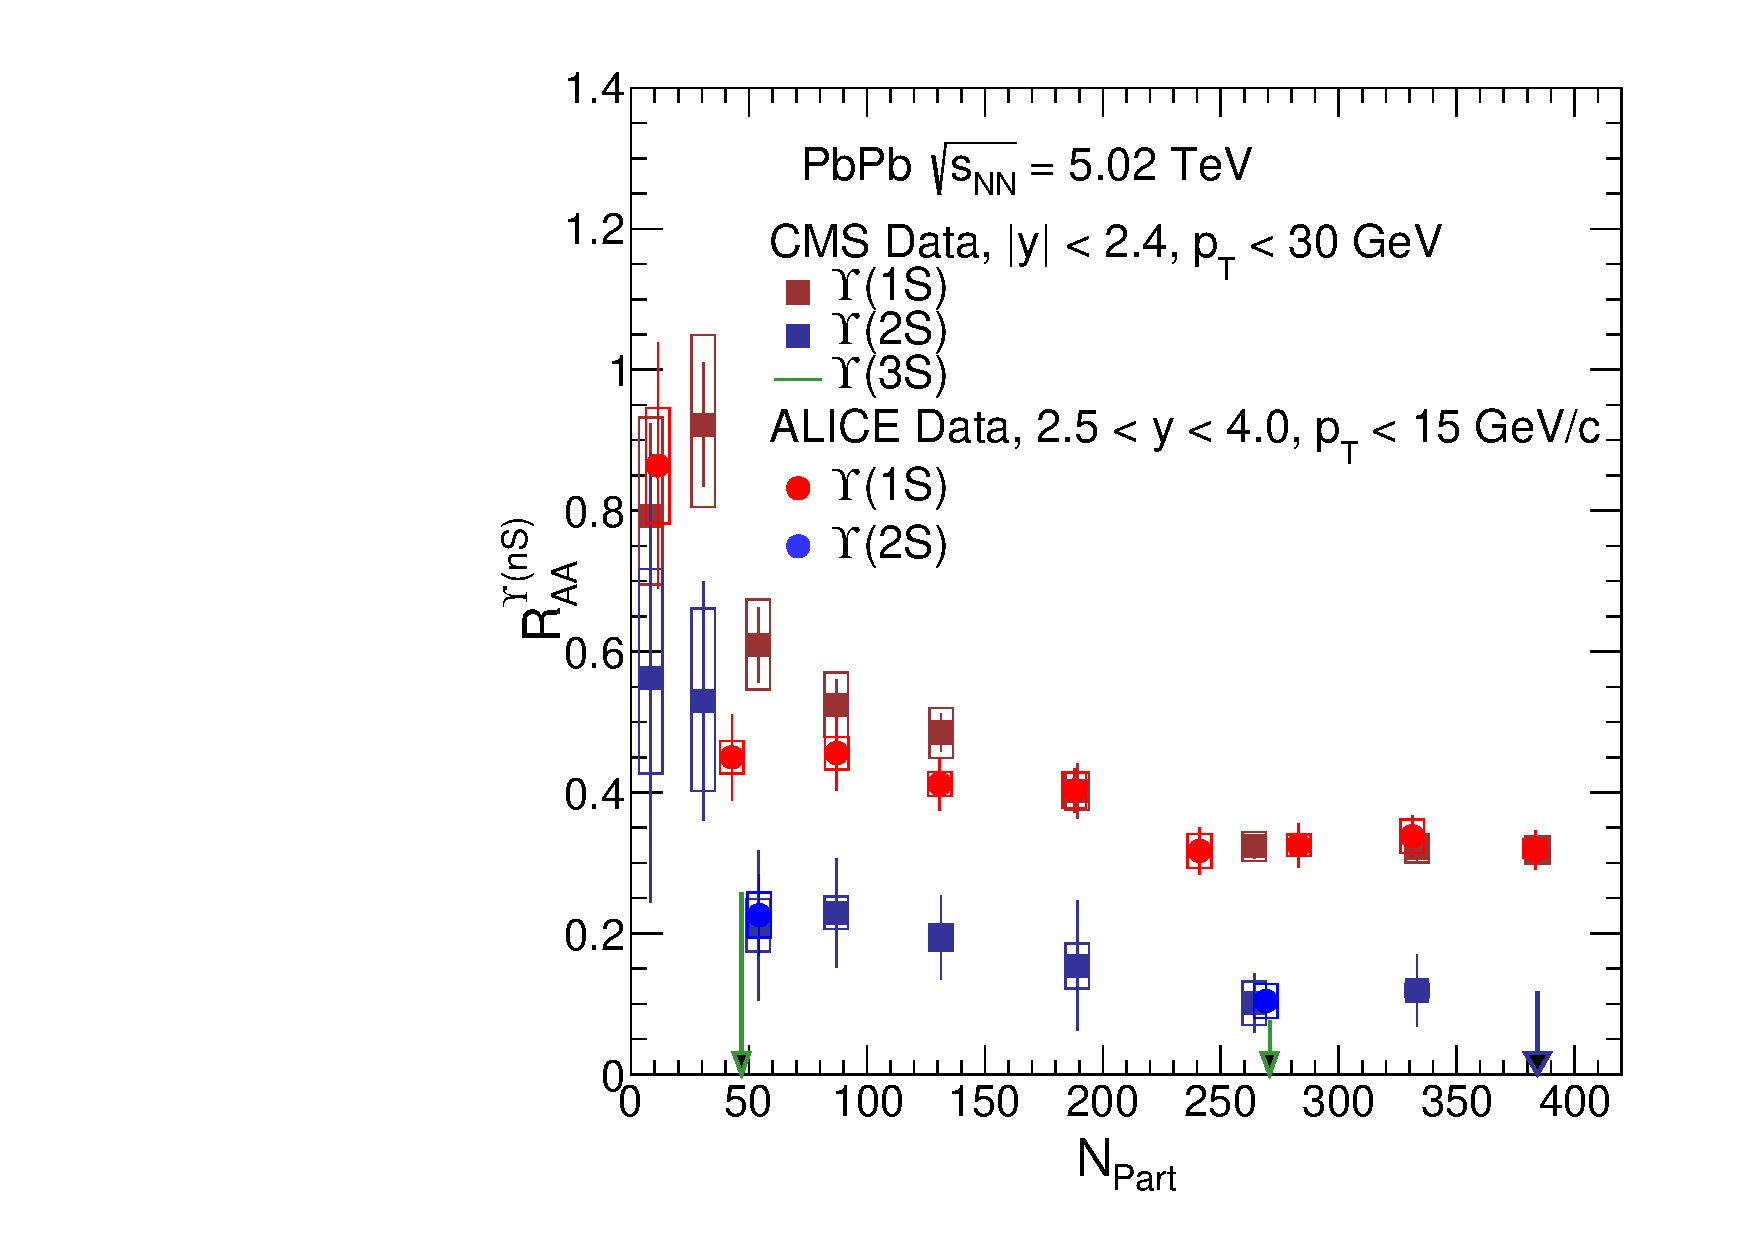
\includegraphics[width=0.49\textwidth]{Figures/ExpOverview/Fig_LHC_YnSRAANPart.pdf}
  %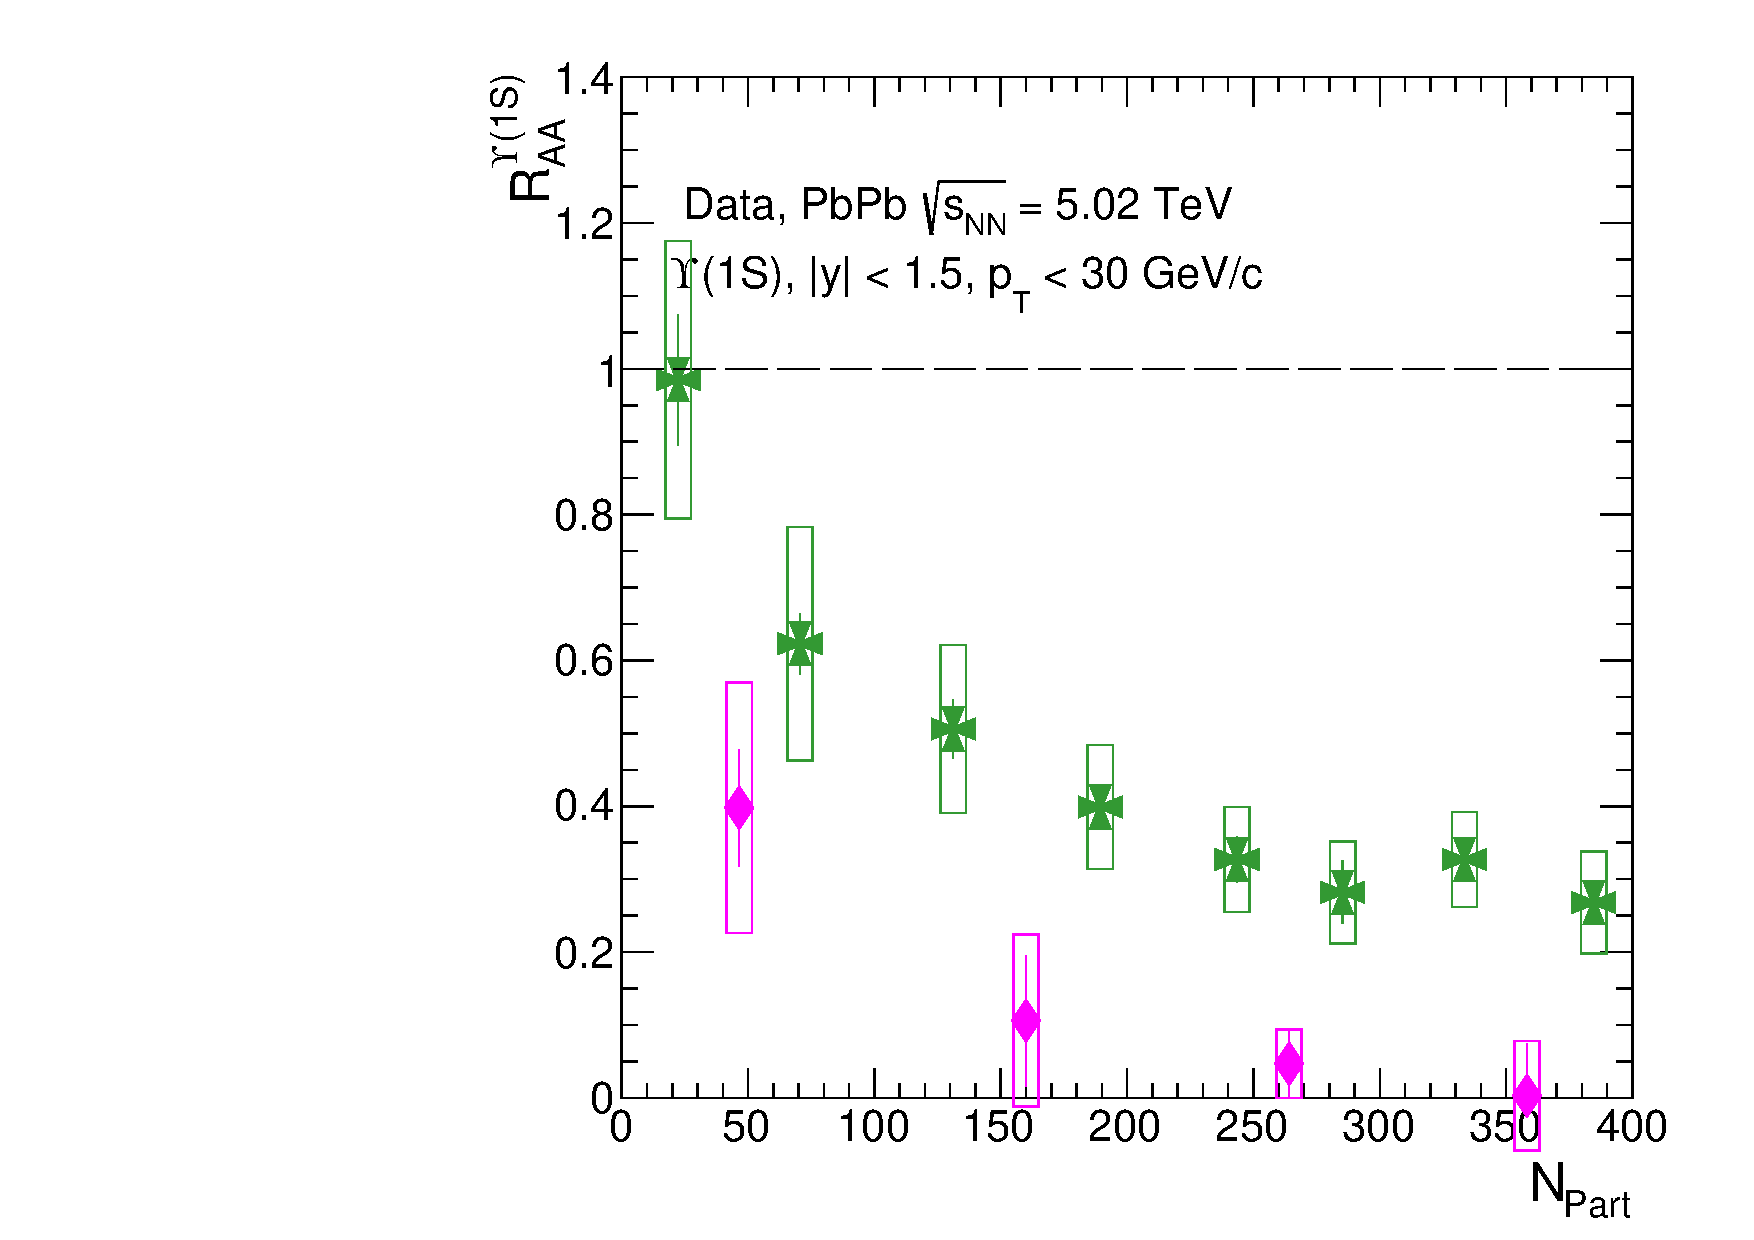
\includegraphics[width=0.49\textwidth]{Figures/ExpOverview/Fig_ATLAS_YnSRAACent_temp.pdf}
  \caption{(Color online) The $\Upsilon$(nS) nuclear modification factor, $R_{AA}$ as a function of N$_{\rm Part}$
    measured by CMS~\cite{CMS:2018zza}, ALICE experiments~\cite{ALICE:2020wwx} and ATLAS experiments~\cite{ALICE:2020wwx}.
    The vertical bars denote statistical uncertainties and the rectangular boxes show the total systematic uncertainties.
  }
  \label{fig:LHCYnSRAANPart}
\end{figure}



\begin{figure}
  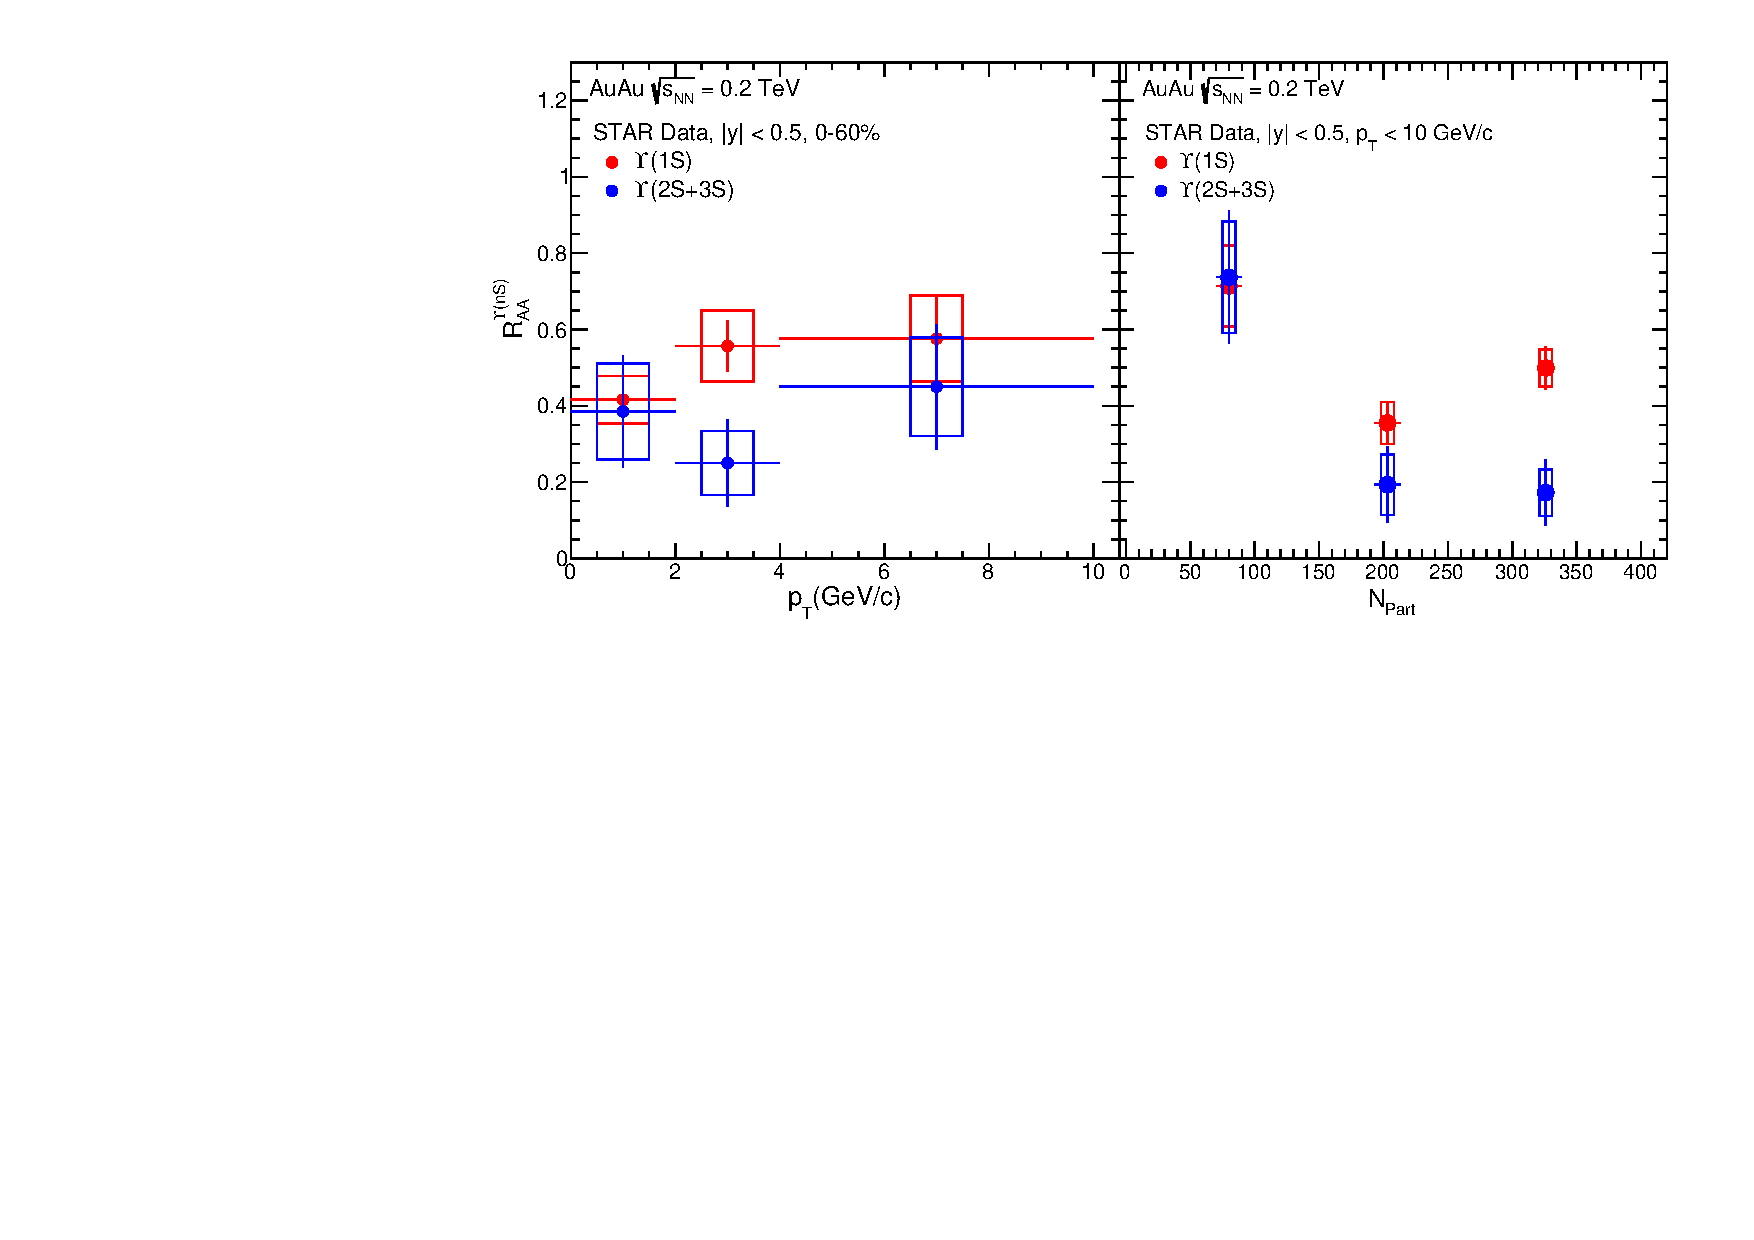
\includegraphics[width=0.99\textwidth]{Figures/ExpOverview/Fig_RHIC_YnSRAAPt.pdf}
  \caption{(Color online) The $\Upsilon$(nS) nuclear modification factor, $R_{AA}$, (a) as a function of transverse momentum $p_{T}$
    and (b) as a function of N$_{\rm Part}$ measured by STAR experiments~\cite{Wang:2019vau}. The vertical bars denote
    statistical uncertainties, and the rectangular boxes show the total systematic uncertainties.
  }
  \label{fig:RHICYnSRAAPtNPart}
\end{figure}



\begin{figure}
  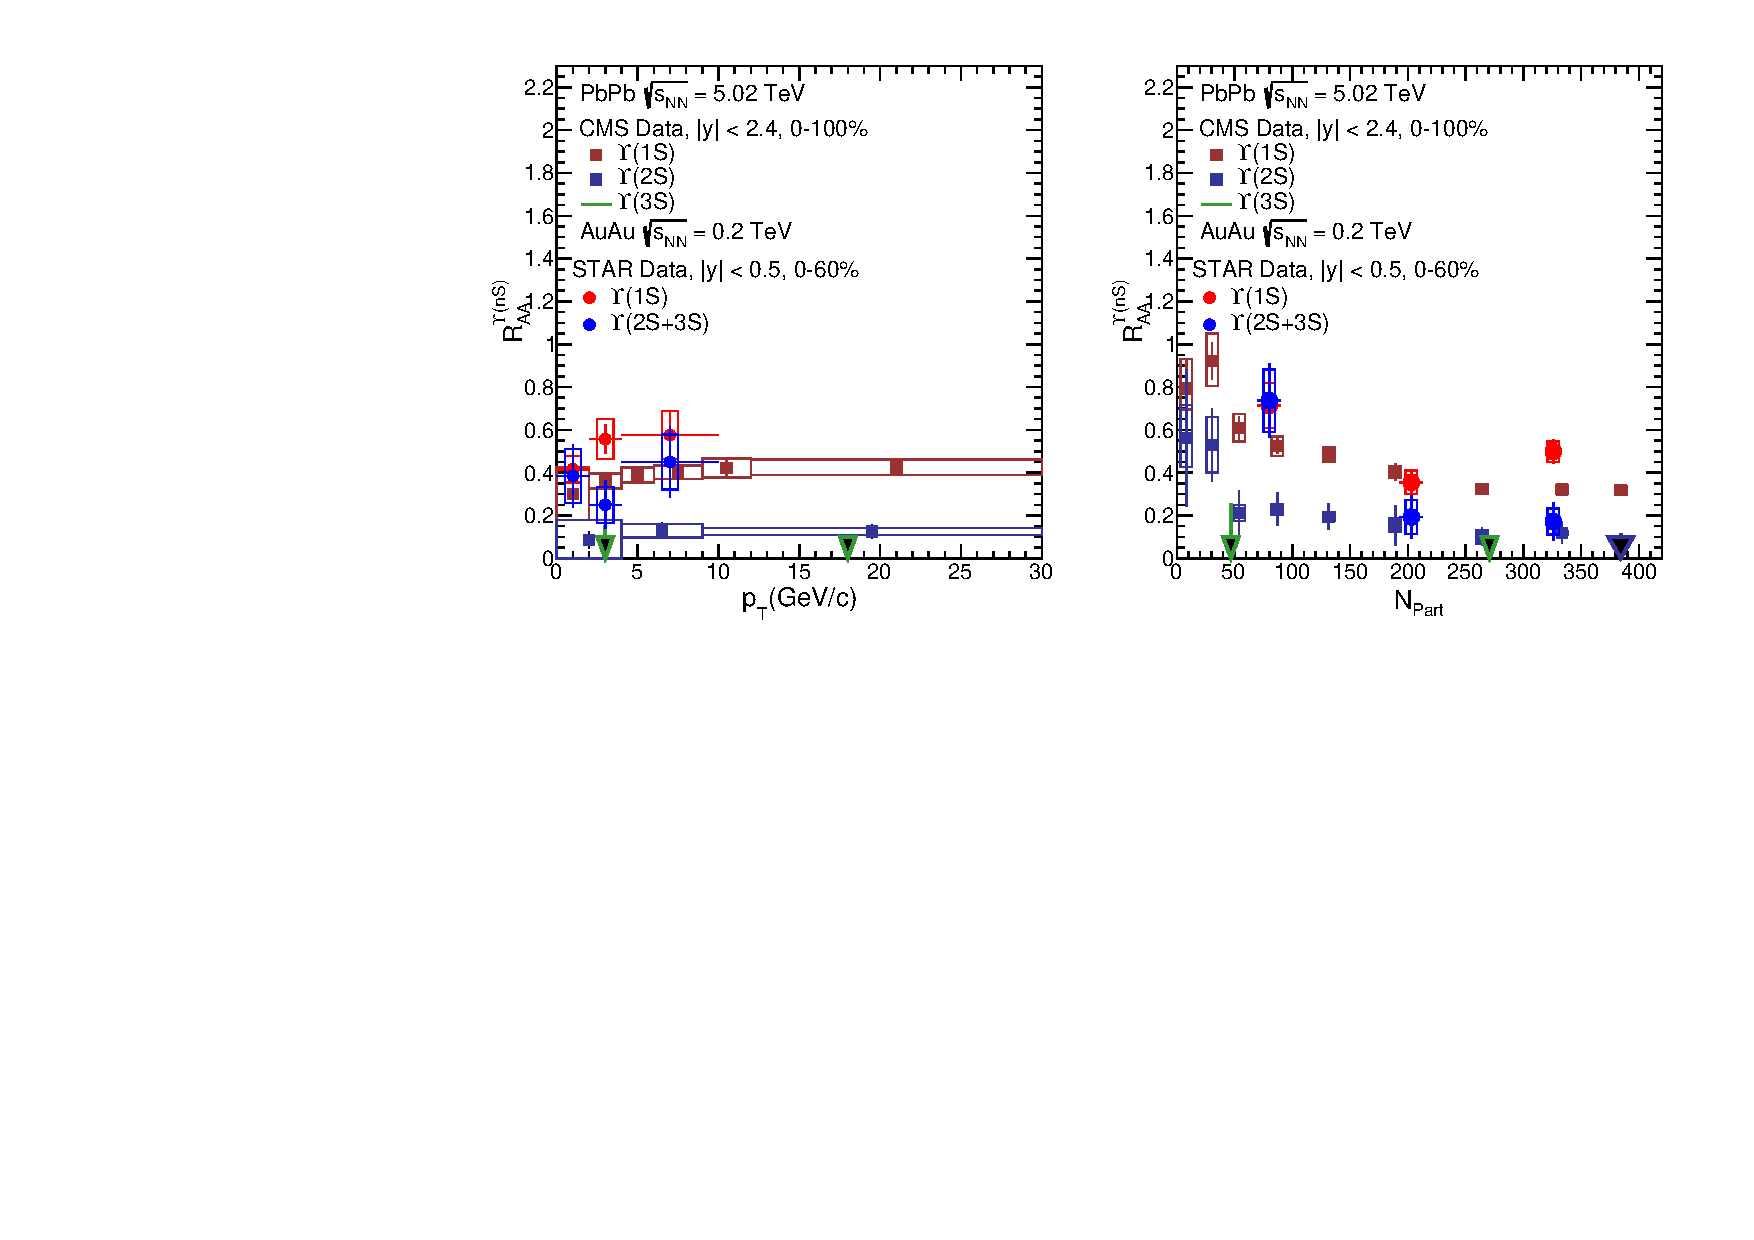
\includegraphics[width=0.99\textwidth]{Figures/ExpOverview/Fig_RHIC_LHC_YnSRAA.pdf}
  \caption{(Color online) The $\Upsilon$(nS) nuclear modification factor, $R_{AA}$, (a) as a function of transverse momentum $p_{T}$
    and (b) as a function of N$_{\rm Part}$ measured by STAR experiments~\cite{Wang:2019vau} at 0.2 TeV and CMS experiment~\cite{CMS:2018zza} at 5.5 TeV.
    The vertical bars denote statistical uncertainties, and the rectangular boxes show the total systematic uncertainties.
  }
  \label{fig:RHICYnSRAAPtNPart}
\end{figure}








\subsection{$\Upsilon$(nS) azimuthal anisotropy}

\begin{figure}
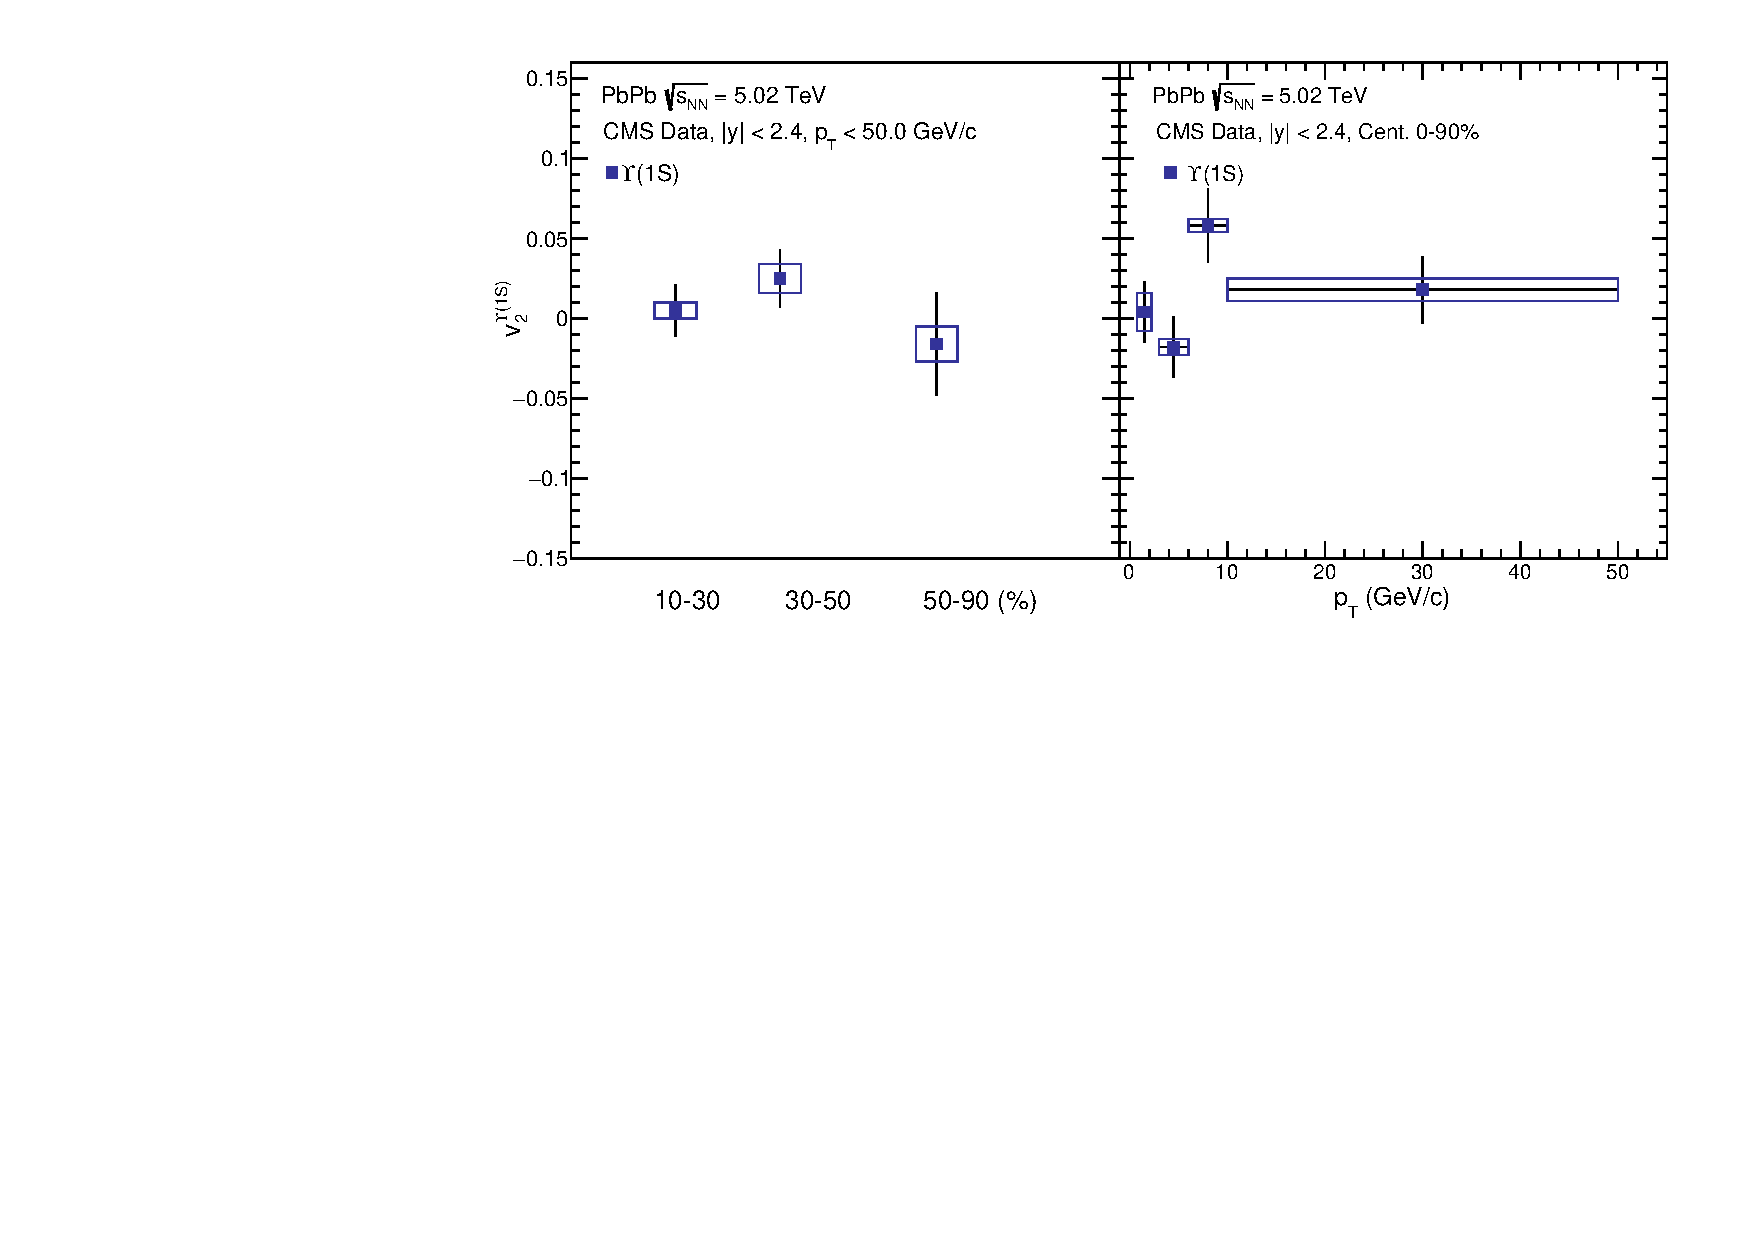
\includegraphics[width=0.99\textwidth]{Figures/ExpOverview/Fig_CMS_Y1S_5TeV_V2.pdf}
\caption{(Color online) The $\Upsilon$(1S) azimuthal anisotropy (v$_{2}$) (a) as a function of collision centrality and 
  (b) as a function of transverse momentum $p_{T}$~\cite{CMS:2020efs}. The vertical bars denote statistical uncertainties,
  and the rectangular boxes show the total systematic uncertainties.
}
\label{fig:Upsilon1SV2CMS}
\end{figure}



The CMS experiment measured v$_{2}$ coefficients for $\Upsilon$(1S) and $\Upsilon$(2S) mesons in PbPb collisions
at a nucleon-nucleon center-of-mass energy of 5.02TeV. Figure~\ref{fig:Upsilon1SV2CMS} shows the $\Upsilon$(1S) azimuthal
anisotropy (v$_{2}$) (a) as a function of collision centrality and (b) as a function of transverse momentum $p_{T}$ measured
by CMS experiment at LHC~\cite{CMS:2020efs}. The p$_{T}$ integrated results
shown in Fig.~\ref{fig:Upsilon1SV2CMS} (a) for three centrality intervals are consistent with zero within the statistical
uncertainties. The average v$_{2}$ values in the 10-90$\%$ centrality interval measured by CMS experiment are found to
be 0.007$\pm$0.011(stat)$\pm$0.005(syst) for $\Upsilon$(1S) and -0.063$\pm$0.085(stat)$\pm$0.037(syst) for $\Upsilon$(2S).   
The p$_{T}$ dependence of $\Upsilon$(1S) meson v$_{2}$ values is measured for the 10-90$\%$ centrality interval.
The v$_{2}$ values are consistent with zero in the measured p$_T$ range, except for the 6$<$p$_{T}<$10 GeV/c interval that
shows a 2.6$\sigma$ deviation from zero. 

\begin{figure}
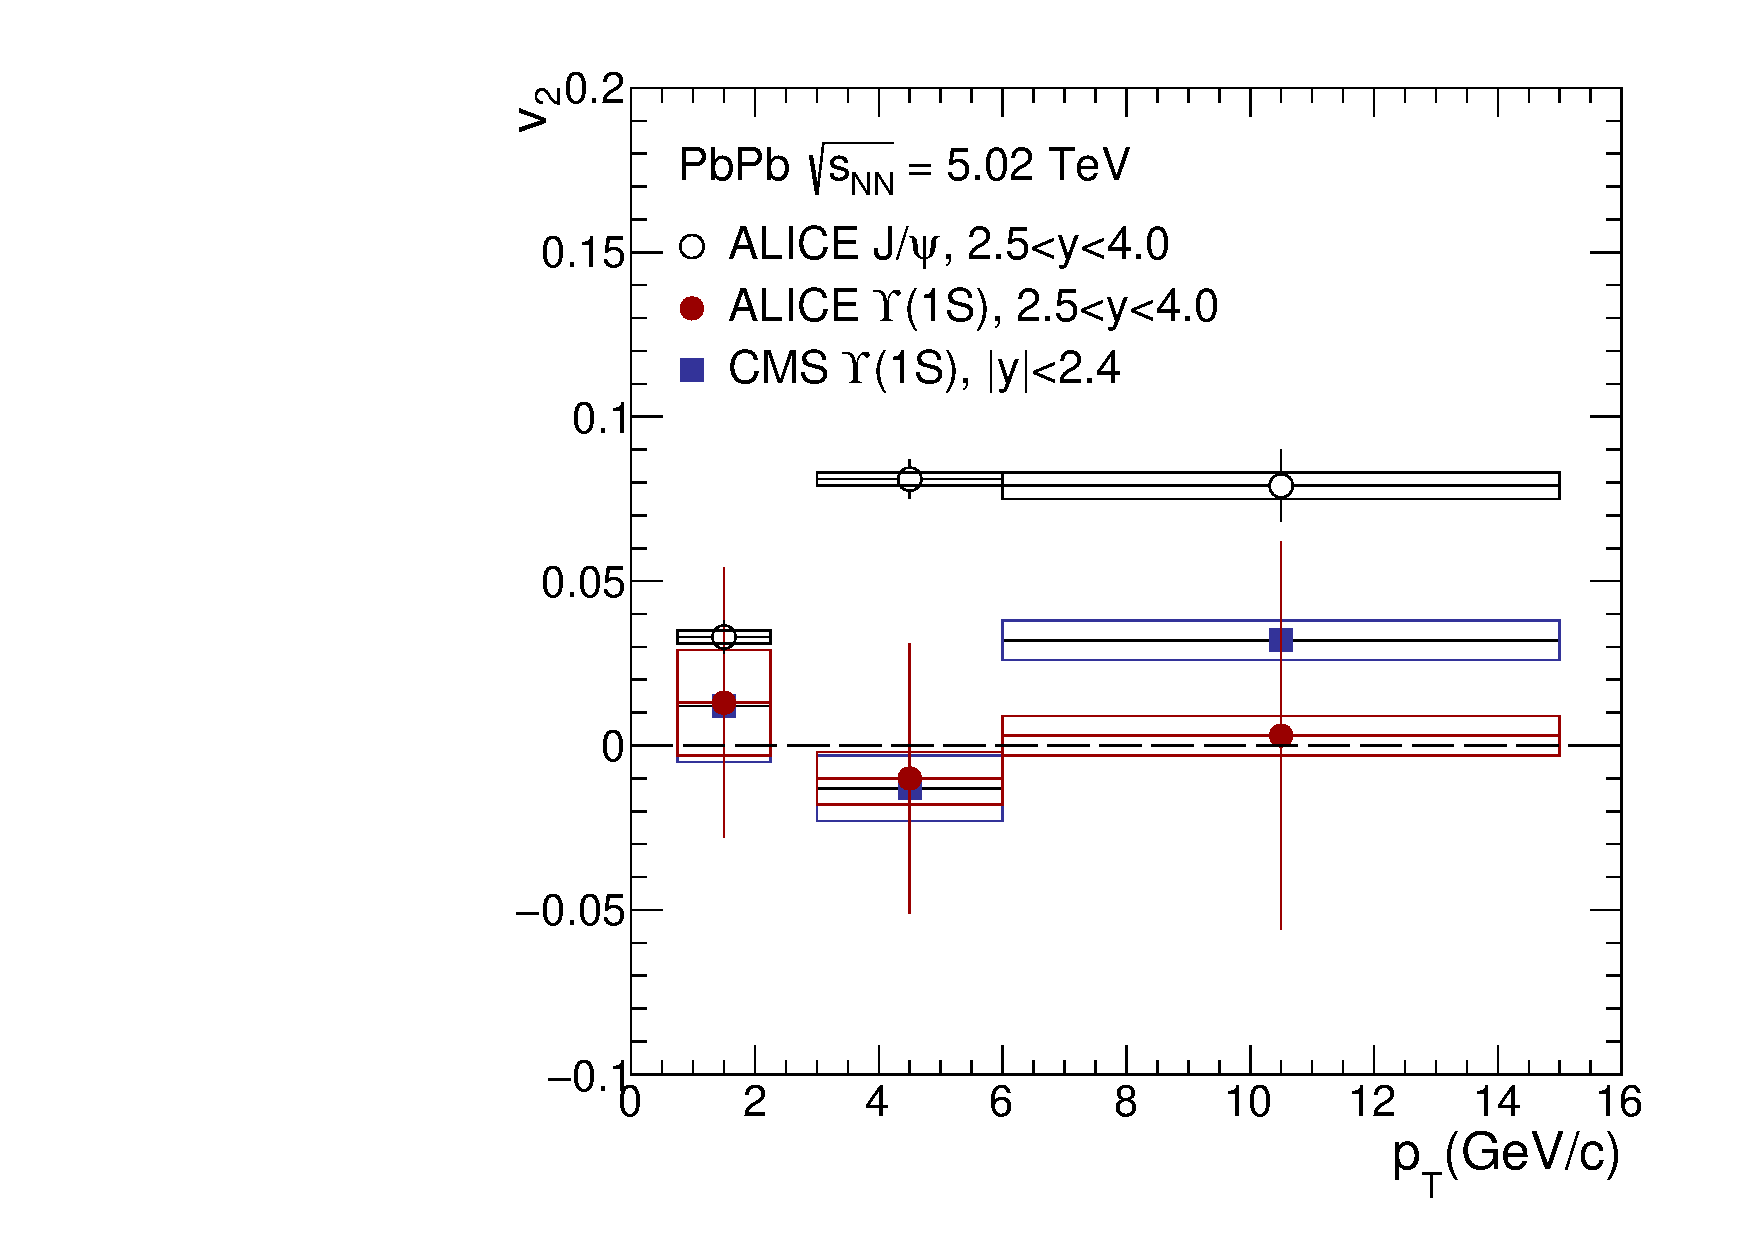
\includegraphics[width=0.49\textwidth]{Figures/ExpOverview/Fig_CMS_ALICE_Y1S_5TeV_V2.pdf}
\caption{(Color online) The v$_{2}$ for $\Upsilon$(1S) mesons as a function of p$_{T}$ in the rapidity range |y|$<$2.4 measured by
  CMS experiment~\cite{CMS:2020efs} compared with the ALICE results for $Upsilon$(1S) and J/$\psi$ mesons measured
  in 2.5$<$y$<$4~\cite{ALICE:2019pox}. The vertical bars denote statistical uncertainties,
  and the rectangular boxes show the total systematic uncertainties.
}
\label{fig:Upsilon1SV2Compare}
\end{figure}

Figure~\ref{fig:Upsilon1SV2Compare} shows the p$_{T}$ differential results for v$_{2}$ of $\Upsilon$(1S)
mesons measured by CMS experiment along with the measurements of v$_{2}$ for $\Upsilon$(1S) and J/$\psi$
from ALICE in the same p$_{T}$ (0-15 GeV/c) and centrality (5-60$\%$) interval. The measurements from CMS
and ALICE are done in complementary rapidity ranges. The $\Upsilon$(1S) V$_{2}$ is consistant with zero while
the J/$\psi$ meson measured by ALICE in same kinematic conditions have finite v$_{2}$. Together, the CMS and ALICE
results indicate that the geometry of the medium has little influence on the $\Upsilon$(1S) yields and recombination is
not a dominant process in the production of this meson. The results also indicate that the path-length depen-dence of
$\Upsilon$(1S) suppression is small.



\subsection{$\Upsilon$(nS) R$_{pA}$ }

\begin{figure}
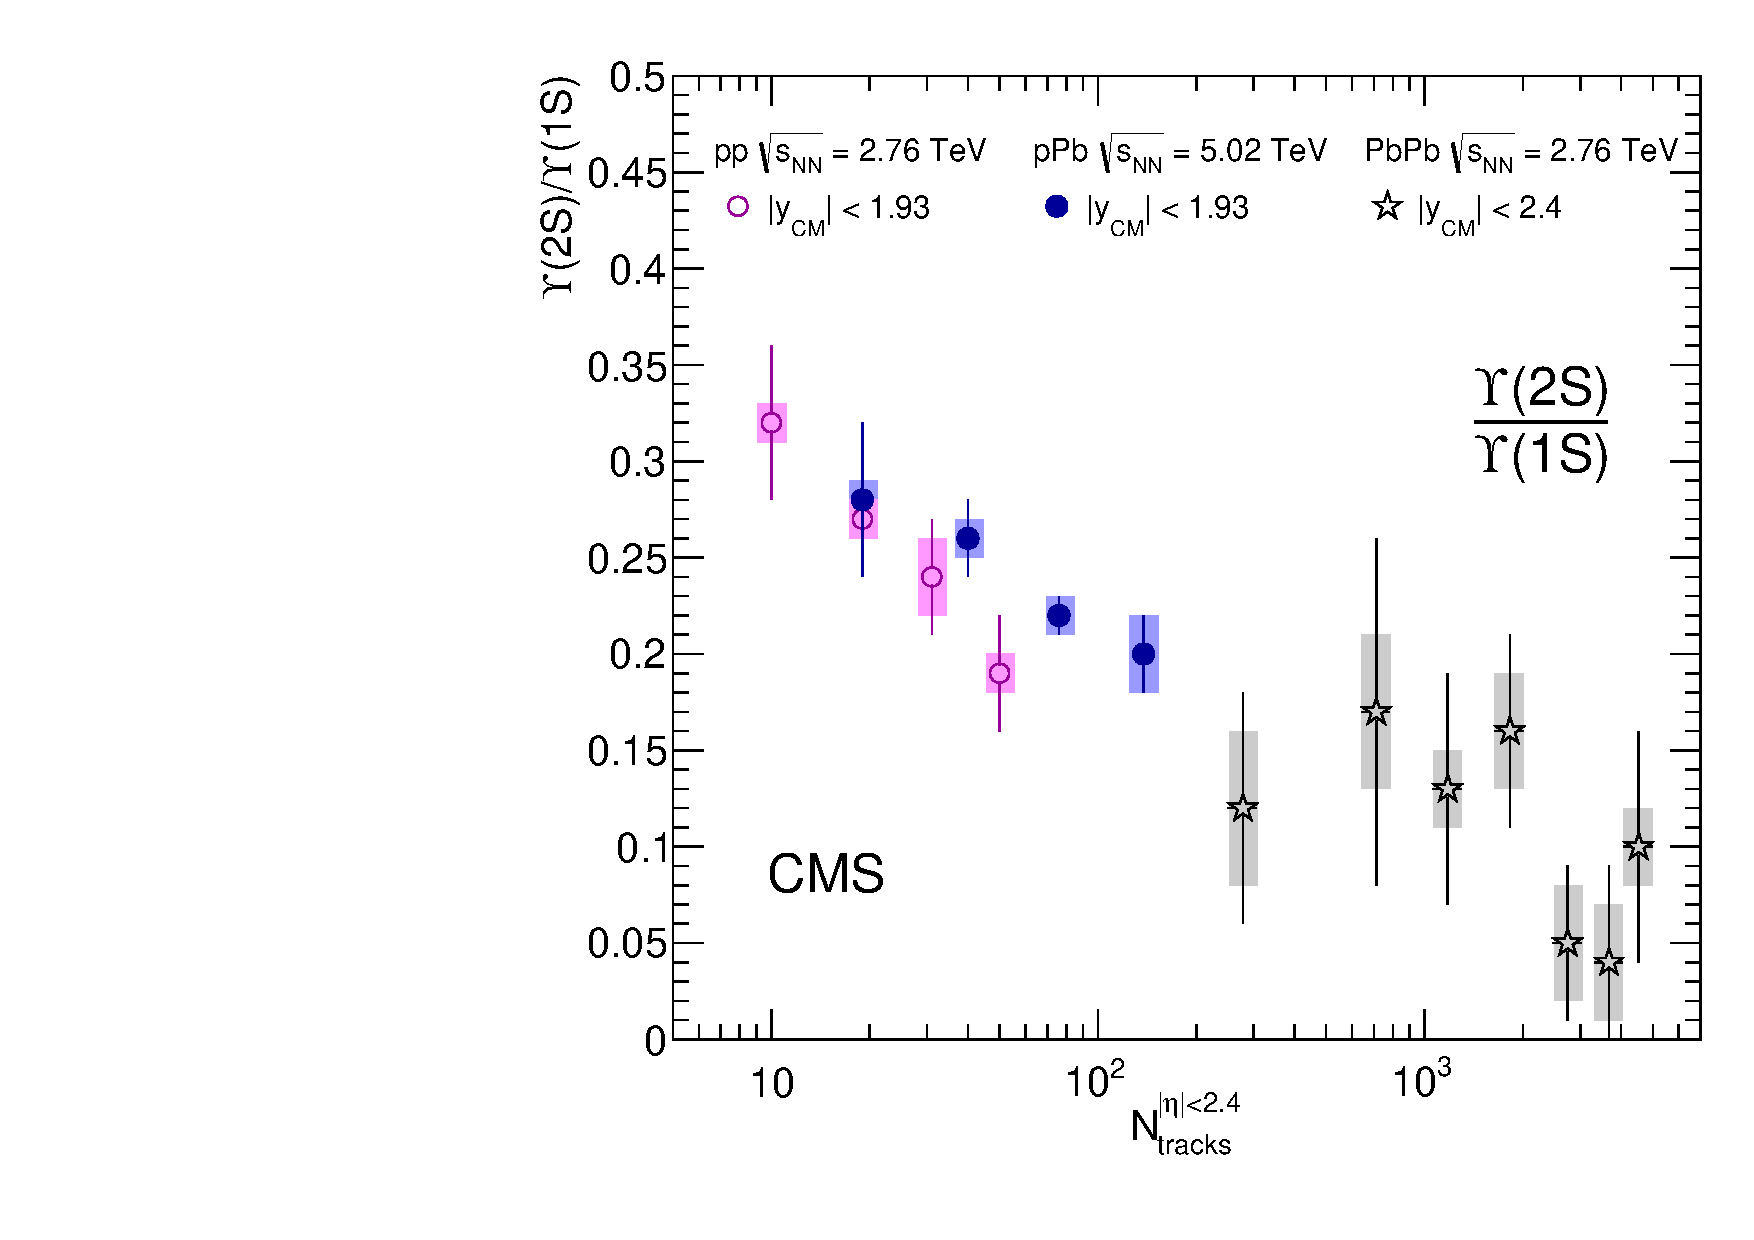
\includegraphics[width=0.49\textwidth]{Figures/ExpOverview/Fig_trk_pPb.pdf}
\caption{(Color online) pPb
}
\label{fig:UpsilonpPb}
\end{figure}
